\section{Bridging Looplets and Finch: The Tensor Interface}
%
The Finch language provides descriptions of computations that iterate over a subset of a regular grid that is lexicographically ordered.
%
At this point, the reader might believe that compilation of a Finch program simply involves simply replacing for loops over a range with for loops over iterators, but Finch programs and data structures are sufficiently flexible that this impossible.
%
First, the Finch language interacts with multi-dimensional tensors whereas the Looplet abstraction is best suited towards iterators over a single dimension.
%
We require a bridge between the single dimensional iterators created from looplets and the mutli-dimensional abstractions common to tensor compilers.
%
Second, since the iteration order of a Finch program might not match that of a data structure (a discordant traversal), different iterators need to be requested for the same data depending on the traversal order of the program.
%
So we require a bridge that can provide different iteration orders depending on the context.
%
Third, since Finch programs can read and write to the same data, multi-dimensional tensors need to provide iterators for reading and writing as well as machinery to manage transition between these states.

\begin{wrapfigure}{R}{0.5\linewidth}
    \centering
    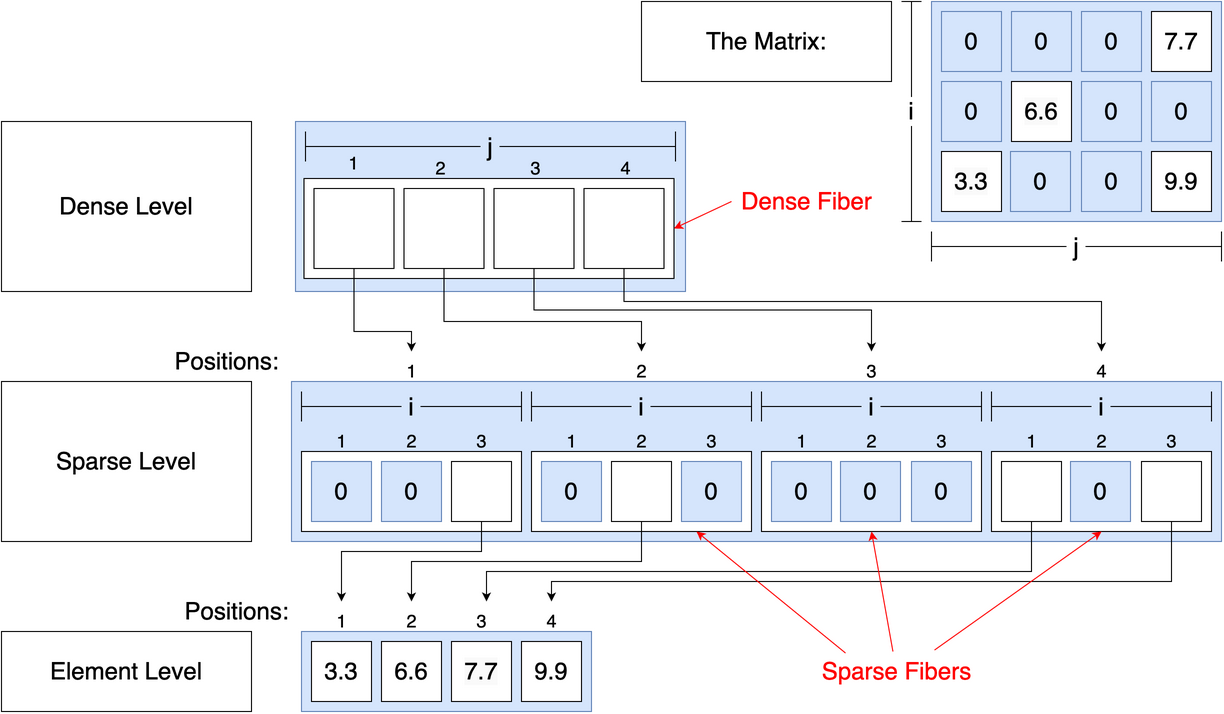
\includegraphics[width=\linewidth]{LevelsVsFibers-matrix.png}
    %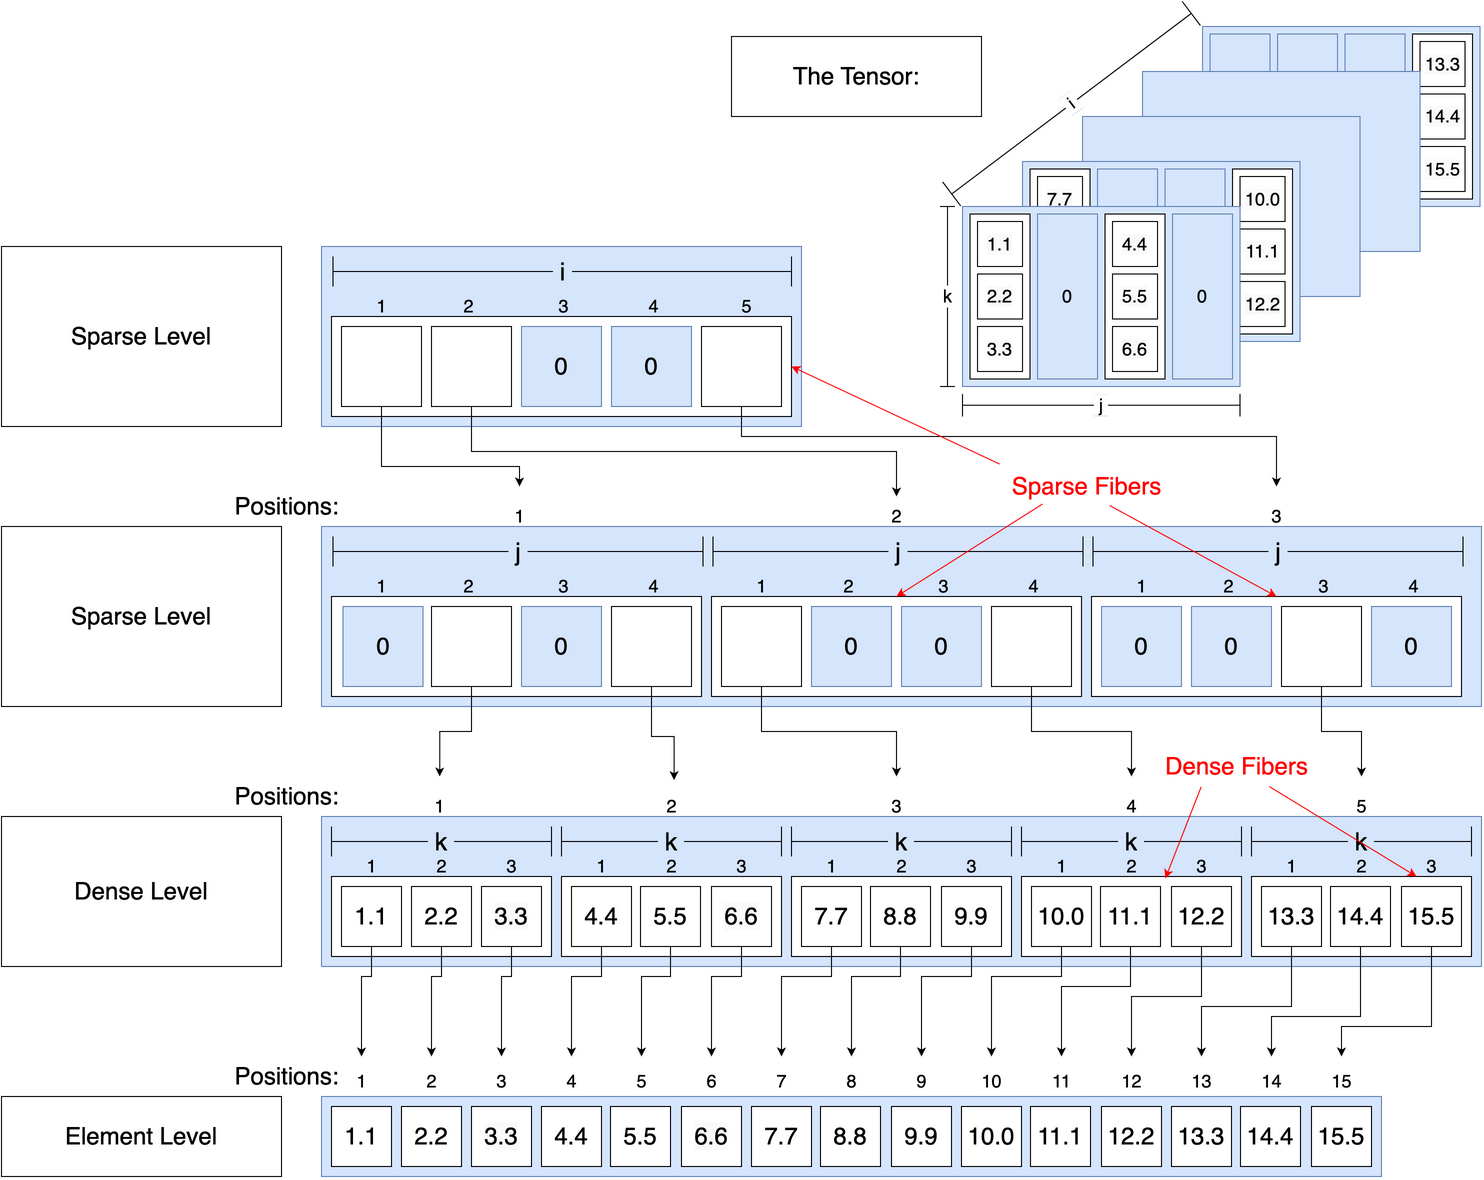
\includegraphics[width=0.5\linewidth]{LevelsVsFibers-tensor.png}
    \caption{Levels in the fiber tree representation of a sparse matrix in CSC format, with a dense outer level and a sparse inner level. The element level holds the leaves of the tree.}
    \label{fig:levelsvsfibers}
\end{wrapfigure}

To build our bridge, we embrace a set of abstractions: level formats/Fiber Trees, iteration context dependent instantiation of iterators, and tensor life cycles.
%
Our first abstraction mostly already exists in the literature: a manner of specifying a data structure for a multi-dimensional tensor out of data structures for single dimensional tensors~\cite{sze2017efficient,chou2022compilation, chou2018format}.
%
We recapitulate the essential details here.
%
Our next two abstractions add to to the first by providing a mechanism to use data structures generated by the first abstraction in a greater variety of contexts while maintaining per-dimension encapsulation of array data structures.
%
We introduce an interface to instatiate iterators in a variety of contexts in our programs and we introduce the lifecycle interface to manage when we read and write to multi-dimensional iterators.
%
These interfaces add to the level abstraction, expanding the types of data that they can express via mapping to looplets and expanding the contexts in which they can be used.
%
Previous efforts to compile a greater variety of sparse array programs left these bridges untouched ~\cite{henry_compilation_2021, won2023unified, senanayake2020sparse}.

%What needs to be said about the tensors? It's basically a few main points:
%1. (DONE) What is the level abstraction 
%2. (Done) We have identified 8 key level structures to represent most combinations of runs or pinpoints.
%2. (Done) a. beautiful figure with datas as rows of larger structures
%2. b. How do we write to each of these, in order? Randomly? random access? several important datastructures that show up along the way.
%3. What is "Unfurling"? and how does it help us represent each structure? refer to looplet decompositions of each case in the earlier figure
%4. (Done) What are lifecycles? How do lifecycles help us keep sane? Why are they necessary for correctness?

\subsection{Level Abstraction}

Fiber-tree style tensor abstractions have been the subject of extensive study
\cite{sze2017efficient, chou2022compilation, chou2018format}.  The underlying
idea is to represent a multi-dimensional tensor as a nested vector
datastructure, where each level of the nesting corresponds to a dimension of the
tensor. Thus, a matrix would be represented as a vector of vectors. This kind of
abstraction lends itself to representing sparse tensors if we vary the type of
vector used at each level in a tree. Thus, a sparse matrix might be represented
as a dense vector of sparse vectors. The vector of subtensors in this
abstraction is referred to as a \textbf{fiber}. Prior fiber-tree representations
focus on sparsity (where only the nonzero elements are represented) and treat
sparse vectors as sets of represented points. Since our fiber-tree
represesentation must handle other kinds of structure, such as diagonal,
repeated, or constant values, we instead view each fiber as a mapping from
indices into a space of subfibers.

%From the docs:
%Finch represents tensors hierarchically in a tree, where each node in the tree is a vector of subtensors and the leaves are the elements. Thus, a matrix is analogous to a vector of vectors, and a 3-tensor is analogous to a vector of vectors of vectors. The vectors at each level of the tensor all have the same structure, which can be selected by the user.
%In a Finch tensor tree, the child of each node is selected by an array index. All of the children at the same level will use the same format and share the same storage. Finch is column major, so in an expression A[i_1, ..., i_N], the rightmost dimension i_N corresponds to the root level of the tree, and the leftmost dimension i_1 corresponds to the leaf level.
%We refer to a node in the tree as a subfiber. All of the nodes at the same level are stored in the same datastructure, and disambiguated by an integer position. in the above example, there are three levels: the rootmost level contains only one subfiber, the root. The middle level has 3 subfibers, one for each column. The leafmost level has 12 subfibers, one for each element of the array. For example, the first level is A_fbr.lvl, and we can represent it's third position as SubFiber(A_fbr.lvl.lvl, 3). The second level is A_fbr.lvl.lvl, and we can access it's 9th position as SubFiber(A_fbr.lvl.lvl.lvl, 9). For instructional purposes, you can use parentheses to call a subfiber on an index to select among children of a subfiber.
%When we print the tree in text, positions are numbered from top to bottom. However, if we visualize our tree with the root at the top, positions range from left to right:
%Dense Format Index Tree
%Because our array is sparse, (mostly zero, or another fill value), it would be more efficient to store only the nonzero values. In Finch, each level is represented with a different format. A sparse level only stores non-fill values. This time, we'll use a tensor constructor with sl (for "SparseList of nonzeros") instead of d (for "Dense"):
%CSC Format Index Tree
%Our Dense(SparseList(Element(0.0))) format is also known as "CSC" and is equivalent to SparseMatrixCSC. The Tensor function will perform a zero-cost copy between Finch fibers and sparse matrices, when available. CSC is an excellent general-purpose representation when we expect most of the columns to have a few nonzeros. However, when most of the columns are entirely fill (a situation known as hypersparsity), it is better to compress the root level as well:
%DCSC Format Index Tree
%Here we see that the entirely zero column has also been compressed. The SparseList(SparseList(Element(0.0))) format is also known as "DCSC".
%The COO format is compact and straightforward, but doesn't support random access. For random access, one should use the SparseHash format. A full listing of supported formats is described after a rough description of shared common internals of level, relating to types and storage.
%All levels have a postype, typically denoted as Tp in the constructors, used for internal pointer types but accessible by the function:
%postype(lvl)


Instead of storing the data for each subfiber separately, most sparse tensor
formats such as CSR, DCSR, and COO usually store the data for all fibers in a
level contiguously. In this way, we can think of a level as a bulk allocator for
fibers. Continuing the analogy, we can think of each fiber as being
disambiguated by a \textbf{position}, or an index into the bulk pool of
subfibers. The mapping $f$ from indices to subfibers is thus a mapping from an
index and a position in a level to a subposition in a sublevel.
Figure~\ref{fig:levelsvsfibers} shows a simple example of a level as a pool of fibers.

When we need to refer to a particular fiber at position $p$ in the level $l$, we
may write $fiber(l, p)$. Note that the formation of fibers from levels is lazy,
and the data underlying each fiber is managed entirely by the level, so the
level may choose to overlap the storage between different fibers. Thus, the only
unique data associated with $fiber(l, p)$ is the position $p$.

\subsection{The 8 Key Level Structures}
    \begin{wrapfigure}{R}{.35\textwidth}
        \centering
        \scriptsize
        \begin{tabular}{|c|c|c|c|l|}
            \hline
            \rothead{Sparse} & \rothead{Blocked} & \rothead{Runs} & \rothead{Singletons} & \begin{tabular}{@{}l@{}}\textbf{Corresponding} \\ \textbf{Format}\end{tabular} \\
            \hline
             &  &  &  & Dense \\
            \hline
             &  & \checkmark &  & DenseRLE \\
            \hline
            \checkmark &  &  &  & Sparse \\
            \hline
            \checkmark &  &  & \checkmark & SparsePinpoint \\
            \hline
            \checkmark &  & \checkmark &  & SparseRLE \\
            \hline
            \checkmark &  & \checkmark & \checkmark & SparseInterval \\
            \hline
            \checkmark & \checkmark &  &  & SparseVBL \\
            \hline
            \checkmark & \checkmark &  & \checkmark & SparseBand \\
            \hline
        \end{tabular}
        \caption{All combinations of relevant structural properties and their
        corresponding formats.  Note that blocks and runs need not be considered
        together because we must store a run length for each run, and so there
        isn't a significant storage benefit to combining them. Blocks and
        singletons only make sense in the contex of sparsity, so we don't
        consider them together either. We omit such combinations
        from the exhaustive table.}
        \label{tab:TypesOfStructure}
    \end{wrapfigure}
    The main benefits of specializing to structure come from the following properties of the data:
    \begin{enumerate}
        \item[Sparsity] Sparse data is data that is mostly zero, or some other
        fill value. When we specialize on this data, we can use annihilation ($x
        * 0 = 0$), identity ($x * 1 = 1$), or other constant propagation
        properties ($ifelse(false, x, y) = y$) to simplify the computation and avoid
        redundant work.
        
        \item[Blocks] Blocked data is a subset of sparse data where the nonzeros
        are clustered and occur adjacent to one another. This provides us with
        two opportunities: We can avoid storing the locations of the nonzeros
        individually, and we can use more efficient randomly accessible
        iterators within the block. \cite{im_optimizing_2001, vuduc_performance_2002, ahrens_looplets_2023}.

        \item[Runs] Runs of repeated values may occur in dense or sparse code,
        cutting down on storage and allowing us to use integration rules such as 
        \mintinline{julia}{for i = 1:n; s += x end} $\rightarrow$
        \mintinline{julia}{s += n * x} or code motion to lift operations out of loops \cite{donenfeld_unified_2022,ahrens_looplets_2023}.

        \item[Singletons] When we have only one non-fill region in sparse data,
        we can avoid a loop entirely and reduce the complexity of iteration \cite{ghorbani2023compiling, ahrens_looplets_2023}.
    \end{enumerate}

    In Finch, we have identified 8 key level structures that can represent all
    of the relevant combinations of these properties, summarized in Table
    \ref{tab:TypesOfStructure}. We examine each structure in turn, describing
    some of the key properties and potential use cases of each. In this sense,
    the structures we consider are exhaustive. We can represent a wide variety
    of hierarchical tensor structures by combining these level structures in a
    tree, as shown in Figure~\ref{fig:structuraldiversity}.

    \begin{figure}
        \centering
        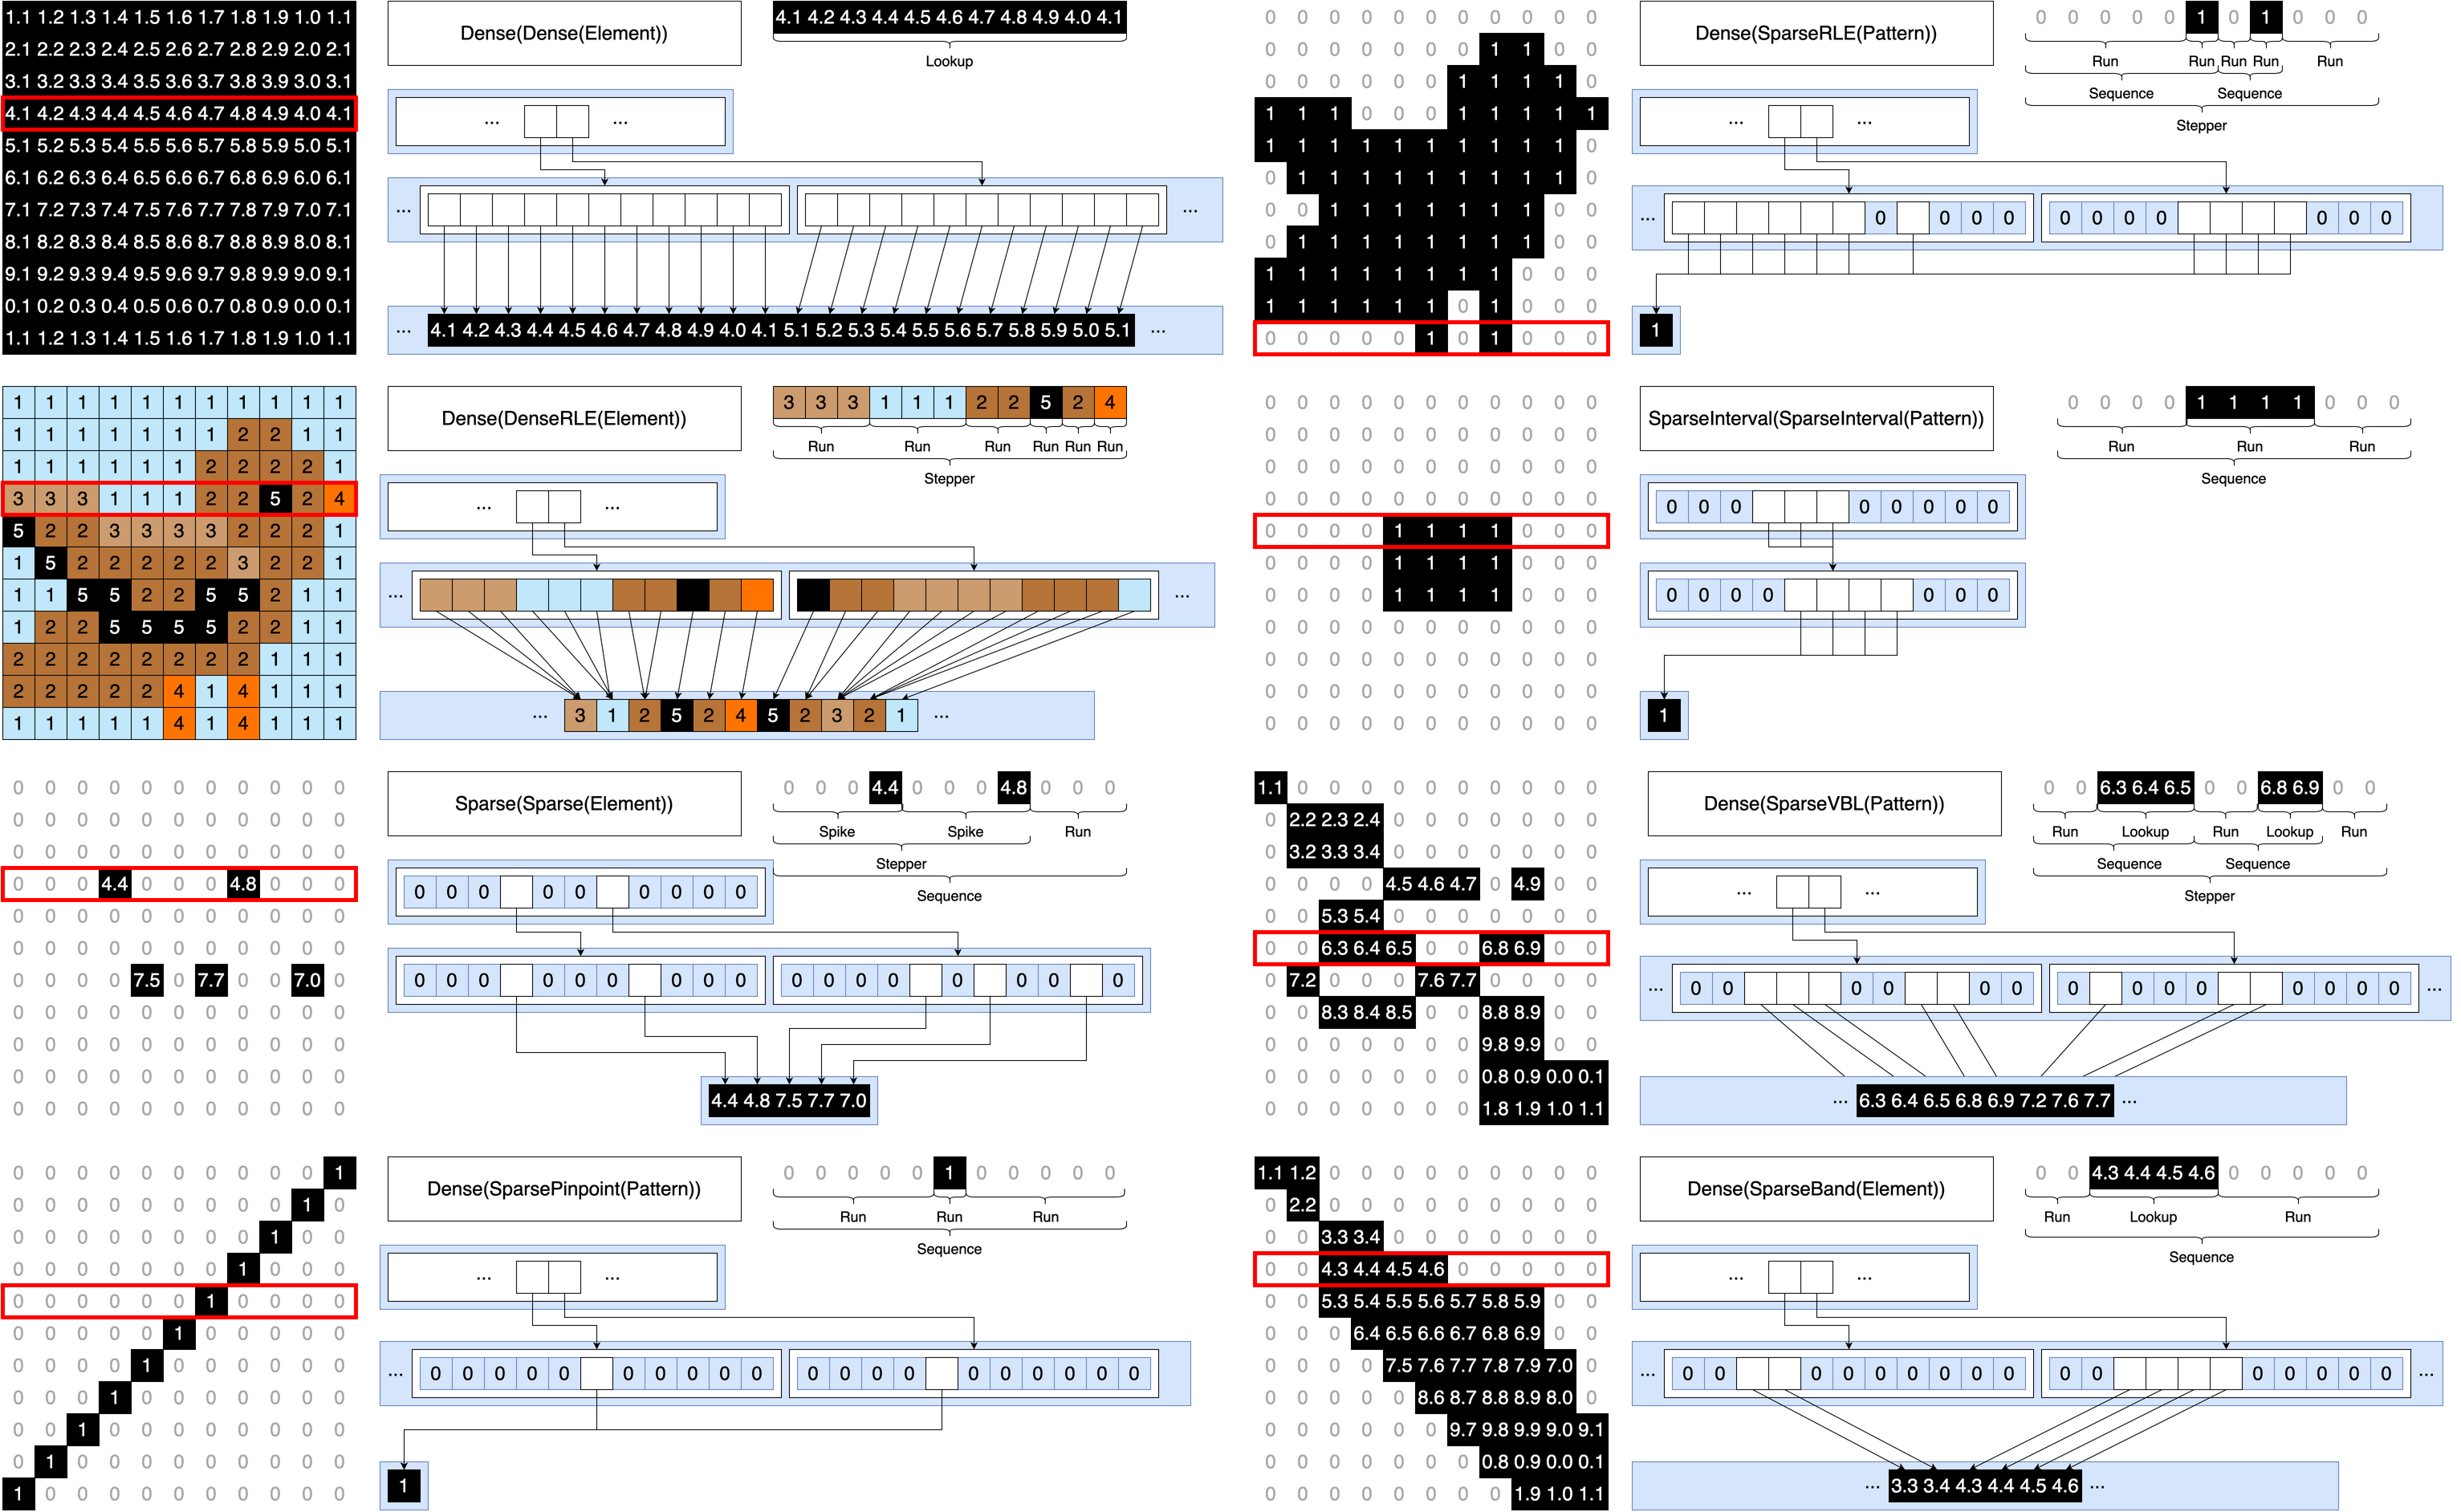
\includegraphics[width=\linewidth]{Structures.png}\hfill%
        \caption{Several examples of matrix structures represented using the
        level structures identified in Table~\ref{tab:TypesOfStructure}.
        Comparing this figure to \cite[Figure 3]{ahrens_looplets_2023}, we see
        that a level-by-level structural decomposition is diagrammed together
        with the Looplets.}
        \label{fig:structuraldiversity}
    \end{figure}

\subsection{Tensor Lifecycle, Declare, Freeze, Thaw, Unfurl}

Our simplified view of a level is enabled by our use of looplets to represent
the structure within each fiber. In fact, our level interface requires only 5
highly general operations, described below.

The first three of these functions, declare, freeze, and thaw, have to do with
managing when tensors can be assumed mutable or immutable. As we use Looplets to
represent iteration over a tensor, we must restrict the mutability of tensors
while we iterate over them. For example, if a tensor declares it has a constant
region from $i = 2:5$, but some other part of the computation modifies the
tensor at $i = 3$, this would result in incorrect behavior. It is much easier to
write correct Looplet code if we can assume that the tensor is immutable while
we are reading from it. Thus, we introduce the notion that a tensor can be in
read-only mode or update-only mode.  In read-only mode, the tensor may only
appear in the right-hand side of assignments. In update-only mode, the tensor
may only appear in the left-hand side of an assignment, either being overwritten
or incremented by some operator.  We can switch between these modes using freeze
and thaw functions. The declare function is used to allocate a tensor,
initialize it to some specified size and value, and leave it in update-only
mode. 

The unfurl function is used to manage iteration over a subfiber. At the point
when it comes time to iterate over a tensor, be in on the left or right hand
side of an assignment, we call the unfurl function to precompute whatever state
and datastructures are necessary to return a looplet nest that would iterate
over that level of a tensor. The unfurl function is called directly before
iterating over the corresponding loop, so it has access to any state variables introduced
by freezing or thawing the tensor.

Our view of a level as a fiber allocator implies an allocation function
$assemble(tns, pos_{start}:pos_{stop})$, which allocates fibers at positions
$pos_{start}:pos_{stop}$ in the level. We don't specify a de-allocation
function, instead relying on initialization to reset the fiber if it needs to be
reused. While all of the previous functions are used to manage the lifecycle and
iteration over a general tensor, the assemble function is quite specific to the
level abstraction, and the notion of positions within sublevels. Note: it was an
intentional choice to hold the parent level responsible for managing the
data of the sublevels, which positions they allocate, etc. This allows the parent
level to reuse allocation logic from internal index datastructures. For example,
a sparse level might use a list of indices to store which nonzeros are present,
and when it comes time to resize that list, it could also call assemble to resize the
sublevel, reducing the number of branches in the code. The assemble function
lends itself particularly to a "vector doubling" allocation approach, which we
have found to be effective and flexible when managing the allocation
of sparse left hand sides. This benefit is made clear in our evaluation section,
where we see that prior systems like TACO do not support all possible loop
orderings and format combinations for sparse matrix multiply because they do
not have a flexible enough allocation strategy, instead using a two-phase approach
which requires computing a complicated closed-form kernel to iterate over the
data twice to determine the number of required output nonzeros.

\begin{figure}
    \raggedright
\paragraph{$declare(lvl, init, dims...)$} Declares the level to hold subtensors
of size $dims$ and an initial value of $init$. Requires the level to be in
read-only mode.
\paragraph{$freeze(lvl)$} Finalizes the updates in the level, and readies the
level for reading. Requires the level to be in update-only mode.
\paragraph{$thaw(lvl)$} Prepares the level to accept updates. Requires the level
to be in read-only mode.
\paragraph{$unfurl(fiber(lvl, pos), ext, mode)$} Unfurls the fiber at position
$pos$ in the level $lvl$ over the extent $ext$. When $mode = \finchread$,
returns a looplet nest over the values in the read-only fiber.  When $mode =
\finchupdate$, returns a looplet nest over mutable subfibers in the update-only
fiber. Often, skipping over mutable locations allows the level to know which
locations must be stored. Additionally, a dirty bit may be used to communicate
whether the mutable subfiber has been written to, which allows the parent fiber
to know whether the subfiber must be stored explicitly.
\paragraph{$assemble(lvl, pos_{start}, pos_{stop})$} Allocates subfibers in the
level from positions $pos_{start}$ to $pos_{stop}$. Usually, this function is
only ever called on unassembled positions, but some levels (such as dense levels
or bytemaps) may support reassembly.
\caption{The five functions that define a level.}
\end{figure}

\subsection{Level Formats}
Having described the 8 basic level structures and the functions that define a
level format, we can describe the concrete level formats supported by Finch,
some of the challenges in their implementation, and how we overcome them. Note
that these formats are not meant to be exhaustive; we will later give
recommendations for additional level formats to be implemented and explain how
users can also add their own custom formats. Note that all of the levels below store their shape and a sublevel.

\begin{enumerate}
\item[Dense]
    The dense format is the simplest format, and simply maps $fiber(l, p)[i]
    \rightarrow fiber(l.lvl, p * l.shape + i)$. This format is used to store dense data,
    and is often a convenient format for the root level of a tensor. Because
    of its simplicity, freezing and thawing the level are no-ops.
\item[DenseRLE]
    The DenseRLE format is used to represent runs of repeated values. Notice
    that a challenge arises when trying to write to a level with runs: it is
    difficult to merge duplicate runs. Such a scenario might arise when merging
    runs of subfibers of length 3, representing colors in an image.  Ideally, we
    would be able to detect duplicate subfibers and merge them on the fly, but
    we cannot determine which subfibers are equal because we cannot read them
    while the sublevel is in update-only mode. Instead, we merge the duplicates
    during the freeze phase. We $freeze$ the main sublevel, $declare$ a separate
    sublevel as a buffer to store the deduplicated subfibers, and we can then
    compare each of the subfibers in the main level, copying the deduplicated
    subfibers into the buffer:
    \begin{enumerate}
        \item[$right$] A vector of indices corresponding to the end of each run in the level
        \item[$ptr$] A vector of delimiters such that $right[ptr[p]:ptr[p+1] - 1]$ is the set of delimiters in the subfiber at position $p$.
        \item[$buf$] A duplicate sublevel, used to store deduplicated subfibers during $freeze$.
    \end{enumerate}
\item[SparseList]
    The sparse list format is the simplest sparse format, and is used to
    construct the popular CSR, CSC, DCSR, DCSC, and CSF formats. The sparse list
    format consists of the following fields:
    \begin{enumerate}
        \item[$idx$] A vector of nonzero indices in the level
        \item[$ptr$] A vector of delimiters such that $idx[ptr[p]:ptr[p+1] - 1]$ is the set of nonzero indices in the subfiber at position $p$.
    \end{enumerate}
    All of Finch's sparse formats use a dirty bit during writing to determine
    whether the sublevel has been modified from it's default fill value and
    thus, whether it needs to be stored.
\item[SparsePinpoint]
    Because the SparsePinpoint format will only ever store one nonzero in each subfiber,
    we do not need the $ptr$ field.
    \begin{enumerate}
        \item[$idx$] A vector of nonzero indices in the level, one for each subfiber
    \end{enumerate}
\item[SparseRLE]
    Similar to the DenseRLE level, but because the runs are stored on top of a background of fill values, we must also store the start of each run.
    \begin{enumerate}
        \item[$left$] A vector of indices corresponding to the beginning of each run in the level
        \item[$right$] A vector of indices corresponding to the end of each run in the level
        \item[$ptr$] A vector of delimiters such that $left[ptr[p]:ptr[p+1] - 1]$ and $right[ptr[p]:ptr[p+1] - 1]$ are the set of delimiters in the subfiber at position $p$.
        \item[$buf$] A duplicate sublevel, used to store deduplicated subfibers during $freeze$.
    \end{enumerate}
\item[SparseInterval]
    Similar to the SparseRLE level, but $ptr$ is redundant because we only store
    one run. We also don't bother with deduplication here as we cannot store any
    intermediate results with duplicates.
    \begin{enumerate}
        \item[$left$] A vector of indices corresponding to the beginning of each run in the level
        \item[$right$] A vector of indices corresponding to the end of each run in the level
    \end{enumerate}
\item[SparseVBL]
    The SparseVBL format is used to represent blocked data. The format consists
    of the following fields:
    \begin{enumerate}
        \item[$idx$] A vector of indices at the end of each nonzero block in the level
        \item[$ptr$] A vector of delimiters such that $idx[ptr[p]:ptr[p+1] - 1]$ is the set of block terminals in the subfiber at position $p$.
        \item[$ofs$] A vector of delimiters such that $ofs[ptr[p] + q]:ofs[ptr[p] + q + 1] - 1$ are the subpositions of block $q$ in subfiber $p$.
    \end{enumerate}
\item[SparseBand]
    Like SparseVBL, but only one block is stored in each subfiber.
        \item[$idx$] The index at the end of the block in the level
        \item[$ofs$] A vector of delimiters such that $ofs[p]:ofs[p + 1] - 1$ are the subpositions of the block in subfiber $p$.
\end{enumerate}

\help{we need also to talk about pattern and element}

\subsection{Flexible Level Formats}
The levels we described in the previous section are all oriented towards bulk,
sequential creation of formats. However, when users want to be able to write out
of order (which is a common requirement arising from loop order or from the
problem itself, it occurs in our spgemm algorithms and our histogram example in
the evaluation section), we must use more complicated datastructures like hash
tables and trees to support the random access. Because these datastructures are
more complex and have a higher implementation burden and performance overhead,
we only support random access construction of sparse or dense structures.  We
can use these two more general structures as intermediates to convert to our
more specialized structures later.

\begin{enumerate}
\item[SparseHash]
    The sparse hash format uses a hash table to store the locations of nonzeros,
    and sorts the unique indices for iteration during the freeze phase. This
    allows for efficient random access, but not incremental construction, as the
    freeze phase runs in time proportional to the number of nonzeros in the
    entire level.
    \begin{enumerate}
        \item[$idx$] A vector of nonzero indices in the level
        \item[$ptr$] A vector of delimiters such that $idx[ptr[p]:ptr[p+1] - 1]$ is the set of nonzero indices in the subfiber at position $p$.
        \item[$tbl$] A hash table used for construction of the level.
    \end{enumerate}
\item[SparseBytemap]
    The SparseBytemap format uses a bytemap to store which locations have been
    written to. Unlike the SparseHash format, the bytemap assembles the entire
    space of possible subfibers. This accelerates random access in the format,
    but requires a high memory overhead. Because we don't want to reallocate all
    of the memory in each iteration, the declaration of this format instead
    re-assembles only the dirty locations in the tensor. This format is
    analogous to the default workspace format used by TACO.
    \begin{enumerate}
        \item[$idx$] A vector of nonzero indices in the level
        \item[$ptr$] A vector of delimiters such that $idx[ptr[p]:ptr[p+1] - 1]$ is the set of nonzero indices in the subfiber at position $p$.
        \item[$tbl$] A dense array of booleans used to mark dirty locations in the tensor.
    \end{enumerate}
\end{enumerate}

As future work, we also recommend the implementation of a tree-based format, as
this would enable incremental construction. Currently, the cost of freezing and
thawing is usually proportional to the number of stored fibers, so an operation
that sets a single value in a tensor would be prohibitively expensive (i.e.
$A[3, 4] = 3.14$). We would also recommend supporting SparseRLE as an
intermediate randomly accessible structure, because (unlike blocks or
singletons), runs have asymptotic benefits. However, these cases were not
necessary for our case studies.

\subsection{Scalars}

\subsubsection{Sparse Scalars}
\subsubsection{Early Break Scalars}